% !TeX root = TGGBenutzerhandbuch_main.tex
\chapter{Einführung}

\section{Motivation}
Der TGG Editor wurde an der Technischen Universität Berlin im Rahmen des Projekts \emph{Visuelle Sprachen} im Wintersemester 2011/2012 von den Studenten Daniel Binanzer, Waka Nagasawa, Frank Röske und Sebastian Schasse als Eclipse Plugin in Java entwickelt und baut auf die Plugins EMF\index{EMF}, GEF\index{GEF} und MuvitorKit\index{MuvitorKit} auf. Der TGG Editor ist eine Spezialisierung des ebenfalls in einem vorhergehenden Projekt \emph{Visuelle Sprachen} entwickelten Henshin Editors\index{Henshin Editor}\footcite[][\url{http://tfs.cs.tu-berlin.de/henshin/}]{henshinwebsite}
%\footnote{Henshin Editor Webseite - http://tfs.cs.tu-berlin.de/henshin/}
. Mit dem TGG Editor lassen sich grafische Tripel Graph Grammatiken\index{Tripel Graph Grammatik} für beliebige Sprachen erzeugen und testen. Die entwickelten TGGs werden im TGG Editor als Instanzen des Henshin EMF Modells mit zusätzlichen Layoutinformationen gespeichert. Die verwendeten Quell- und Zielsprachen müssen als EMF Modell definiert sein und importiert werden. TGGs ermöglichen die formal korrekte Transformation von einer Quell- in eine Zielsprache. Beispiele für Quell- und Zielsprachen sind grafische Sprachen wie UML Klassendiagramme oder Relationale Datenbankmodelle, aber auch textbasierte Sprachen wie COBOL und C++. Der hier vorgestellte TGG Editor unterstützt allerdings nur visuelle Sprachen. Die Entwicklung der Transformationsregeln in einer TGG sind sehr einfach. Nachdem diese Regeln für die Quell- und Zielsprache erstellt wurden, können mit einem Klick Graphen von einer Quellsprache in die Zielsprache übersetzt werden.


%Das vorliegende Handbuch des TGG Editors enthält die folgenden Teil: Nach dieser Motivation gehen wir in Abschnitt \ref{sec:theorie} auf den theoretischen Hintergrund des Editors ein. In Abschnitt \ref{sec:implementation} wird vor allem das EMF Metamodell des TGG Editors diskutiert. Im darauf folgenden Kapitel \ref{chap:tutorial} wird Schritt für Schritt ein einführendes Beispiel beschrieben. Im letzten Kapitel \ref{chap:kommandos} werden alle Funktionalitäten des Editors erläutert. Außerdem verfügt dieses Handbuch auf Seite \pageref{chap:index} über eine Index, damit Begriffe schnell und einfach nachgeschlagen werden können.
%
%
\section{Formale Spezifikation}\label{sec:theorie}\index{Theorie}
Dieses Kapital umreißt kurz die theoretischen Hintergründe der Graph- und Modelltransformation und der \emph{Tripelgraphgrammatik}\index{Tripelgraphgrammatik} (TGG). Für ein tieferes Verständnis empfiehlt sich eine tiefere Recherche in entsprechender Literatur\footcite{ehrig2006}\footcite{ehrig2009}\footcite{schuerr1995}.

\subsection{Graphen}
Die folgende Definition bezieht sich nur auf gerichtete Graphen, da wir in dem hier vorgestellten Graphtransformation nur mit gerichteten Graphen arbeiten.\\
\ \\
Ein \emph{gerichteter Graph}\index{gerichteter Graph} ist ist ein Quadrupel $(V,E,src,tar)$ wobei $V$ eine Menge von Knoten, $E$ eine Menge von Kanten, $src$ die source-Funktion $src:E\rightarrow V$, die einer Kante einen Startknoten zuordnet, und $tar$ die target-Funktion $tar:E\rightarrow V$, die einer Kante einen Endknoten zuordnet, ist.
\subsection{Typgraph}
\label{subsec:Typgraph}
Ein \emph{Typgraph}\index{Typgraph} ist ein Graph $TG = (V_{TG},E_{TG},src_{TG}, tar_{TG}$, bei dem die Mengen $V_{TG}$ und $E_{TG}$ die Typalphabete für Knoten und Kanten darstellen.\\
\\
Im TGG Editor sind die \emph{Meta-Modelle}\index{Meta-Modell} für Source-, Corresbondence- und Targetgraphen (siehe Tripelgraphgrammatik \ref{subsec:Tripelgraphgrammatik}) sogenannte Typgraphen. Sie ermögliche erst die Erzeugung von \emph{getypten Graphen}\index{getypter Graph}
\subsection{getypter Graph}
Ein \emph{getypter Graph} ist ein Graph, in dem jeder Knoten und jede Kante einen Typen hat.\\
\\
Im TGG Editor sind alle Graphen und Regeln getypte Graphen und müssen verträglich mit dem \emph{Triple-Typgraph}\index{Triple-Typgraph} sein. Dieser Triple-Typgraph wird über die drei Typgraphen, also den Meta-Modellen, für Source, Correspondence und Target erzeugt.
\subsection{Graphmorphismus}
Seien $G_1$ und $G_2$ zwei Graphen mit $G_1 = (V_1,E_1,src_1,tar_1)$ und $G_2 = (V_2,E_2,src_2,tar_2)$. Dann ist $\varphi: G_1 \rightarrow G_2$ ein \emph{Graphmorphismus}\index{Graphmorphismus} mit  $\varphi = (\varphi_V,\varphi_E)$, wenn die Funktionen $\varphi_V: V_1 \rightarrow V_2$ und $\varphi_E: E_1 \rightarrow E_2$ sowohl ziel- ($\varphi_V \circ src_1 = src_2 \circ \varphi_E$) als auch quellerhaltend ($\varphi_V \circ tar_1 = tar_2 \circ \varphi_E$) sind.
\subsection{Regel}
Diese Definition bezieht sich auf getypte Regeln Graphen und Graphmorphismen, da nur diese im TGG Editor verwendet werden.\\
\\
Eine Regel $r$ besteht aus den drei Graphen $L$ (auch \emph{left-hand side}\index{left-hand side}, \emph{Linke-Hand-Seite}\index{Linke-Hand-Seite} oder \emph{LHS}\index{LHS} genannt), $K$ (auch \emph{Klebegraph}\index{Klebegraph} genannt) und $R$ (auch \emph{right-hand side}\index{right-hand side}, \emph{Rechte-Hand-Seite}\index{Rechte-Hand-Seite} oder \emph{RHS}\index{RHS} genannt) und zwei injektiven Graphmorphismen l und r.\\
Im TGG Editor wird der Klebegraph $K$ nur impliziert, da er in unserer Anwendung nur den Schnitt von $L$ und $R$ darstellt.
\subsection{Graphtransformation}
Eine Graphtransformation ist eine auf Regeln basierte lokale Modifikation eines Graphen.
\begin{wrapfigure}{r}{5.5cm}
	\centering
	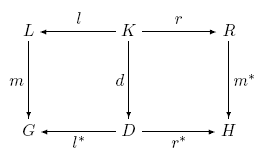
\includegraphics[width=5.5cm]{DoublePushout.PNG}
	\caption{DPO Graph\-transformation}
	\label{fig:DoublePushout}
\end{wrapfigure}

Um eine Graphtransformation mit einer Regel $r$ auszuführen, wird zuerst ein Match $m$ von $L$ im Hostgraph $G$ gesucht. Dabei werden alle Knoten und Kanten aus L auf typgleiche und im gleichen Gefüge zueinander stehende Knoten und Kanten des Graphen $G$ abgebildet.
Im Transformationschritt werden die Elemente aus $L \setminus K$ gelöscht, die Elemente aus $K$ erhalten, und die aus $R \setminus K$  hinzugefügt. Anschließend werden Kanten auf denen die Funktionen $src$ oder $tar$ leere Werte zurückliefern gelöscht.\footnote{Kanten, die keinen Start- oder Zielknoten haben werden auch "`h"angende Kanten"' oder "`dangling edges"' genannt und sind nach Definition des Graphens nicht zul"assig.}

\subsubsection{EMF Besonderheiten}
\emph{Eclipse Modeling Framework}\index{Eclipse Modeling Framework} (\emph{EMF}\index{EMF}) bietet die Möglichkeit, Domain-Modelle zu modellieren. EMF unterscheidet das \emph{Meta-Modell}\index{Meta-Modell} und das aktuelle Modell. Das Meta-Modell stellt die Struktur des Modells dar. Ein Modell ist ein Instanz vom Meta-Modell.\\
EMF hat zwei Meta-Modelle. Eins ist das \emph{Ecoremodell}\index{Ecoremodell}, das Informationen der Klassen enthält, das Andere ist das Genmodell, welches zusätzliche Informationen zur Code-Generierung enthält, z.B. Infomationen über Dateien und Pfade.

EMF bietet das Framework als Plugin an, damit Informationenen des Modells gespeichert werden können. Wenn die EMF Meta-Modelle in TGG-Editor importiert werden, können Instanz-Modelle basierend auf den Meta-Modellen erstellt werden. 
Alle verwendbare Kanten und Knoten für Modelle im TGG-Editor sind durch das importierte EMF Modell definiert.

\subsection{Negative Anwendungsbedingung (NAC)}\label{subsec:NegativeAnwendungsbedingung}
Die Menge \emph{negativen Anwendungsbedingungen}\index{Negative Anwendungsbedingung}\index{NAC}\index{negative application conditions} $N = \lbrace N_1, ..., N_n\rbrace$ über den LHS-Graphen $L$ ist eine Menge partieller Erweiterungen $N_i$ von $L$. Die Menge $N_i \cap L$ wird im TGG Editor über das sogenannte Mapping definiert (siehe \ref{subsubsec:Rule_View-Mapping}). 
Die NAC wird dazu verwendet, die Ausführbarkeit einer Graphtransformation auf das Nichtvorhandensein bestimmter Muster im Graphen zu beschränken. \\
Die negativen Anwendungsbedingungen erweitern die Regeldefinition, sodass ein Match nur noch ausführbar wird, wenn keine der vorhandenen NACs gematcht werden kann. Es gibt auch komplexere Bedingungen, bei denen einzelne NACs über logische Operationen "`AND"' und "`OR"' miteinander verknüpft werden können. Die Implementation des TGG Editors unterstützt nur die Verundung aller NACs. Das heißt sobald eine NAC einer Regel matcht ist diese Regel nicht mehr anwendbar. Formal bedeutet das, dass ein Match $m: L \rightarrow G$  $N$ erfüllt (keine NAC matcht), wenn für $\forall N_i \in N$ gilt, es exisitert kein injektiver Graphmorphismus $q_i:N_i \rightarrow G$ verträglich mit $m$.

\subsection{Tripelgraphgrammatik}\label{subsec:Tripelgraphgrammatik}
Die \emph{Tripelgraphgrammatik (TGG)}\index{Tripelgraphgrammatik}\index{TGG} ist ein Formalismus für regelbasierte Transformation von zwei Graphen oder Modellen mit unterschiedlichen Typisierungen. Modelle werden als Paare von Sourcegraphen und Targetgraphen definiert, die über Correspondencegraphen verbunden werden.
Eine Tripelgraphgramatik $TGG = (TG, S, TR)$ besteht aus einem Tripeltypgraph $TG$, einem Tripelstartgraph $S = \phi$ und einer Menge von Tripleregeln $TR$.

\subsubsection{Tripelgraphen}
Ein \emph{Tripelgraph}\index{Tripelgraph} $g=(G_S \stackrel{s_G}{\longleftarrow} G_C \stackrel{t_G}{\longrightarrow} G_T)$ besteht aus den drei Graphen $G_S$ (Sourcegraph), $G_C$ (Correspondencegraph), $G_t$ (Targetgraph) und den zwei Graphmorphismen $s_G:G_C \to G_S$ und $t_G: G_C \to G_T$. \\
Ein \emph{Tripelgraphmorphismus}\index{Tripelgraphmorphismus} $m =(ms, mc, mt):G \to H$ zwischen zwei Tripelgraphen $G$ und $H$ besteht aus drei Graphmorphismen $m_S: G_S \to H_S$, $m_C: G_C \to H_C$ und $m_T: G_T \to H_T$, so dass $m_S \circ s_G = s_H \circ m_C$ und $m_T \circ t_G = t_H \circ m_C$ gilt.

\autoref{fig:CD2RDBM} zeigt den Tripeltypgraphen für eine Beispielmodelltransformation von Klassendiagrammen zu Datenbankmodellen.

\begin{figure}%{r}{10cm}
	\centering
	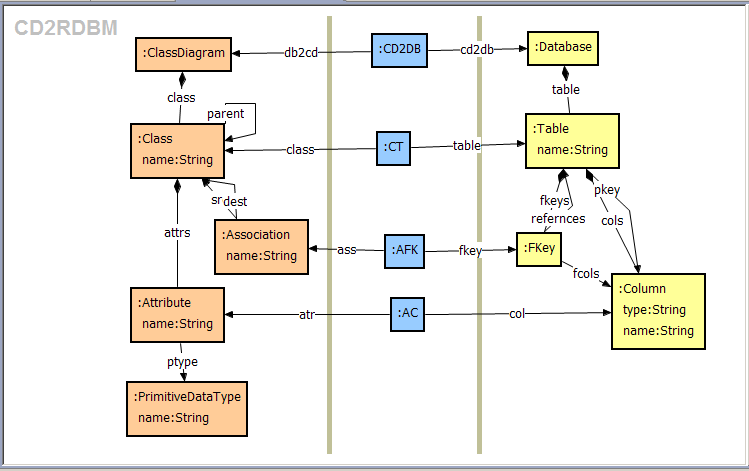
\includegraphics[width=13cm]{CD2RDBM}
	\caption{Beispiel eines Tripelgraphen für CD2RDBM}
	\label{fig:CD2RDBM}
\end{figure}

In der Abbildung steht der Sourcetypgraph $TG_S$ links, der Correspondencetypgraph $TG_C$ in der Mitte und der Targettypgraph $TG_T$ rechts. $TG_S$ definiert die Struktur von Klassendiagrammen und $TG_T$ definiert die Struktur von relationalen Datenbanken. So entspricht eine Klasse aus dem Klassendiagramm einer Tabelle, ein Attribut einer Spalte und eine Assoziation einem Fremdschlüssel.

\subsubsection{Tripelregel}
\emph{Tripelregeln}\index{Tripelregel} bauen Source-, Target-, und Correspondencegraphen synchron auf.
Eine Tripelregel $tr$ ist ein injektiver Tripelgraphmorphismus $tr = (tr_S, tr_C, tr_T): L \to R$ (siehe linken Teil in \autoref{fig:Tripelregel}).
\begin{figure}[h!] %{r}{6cm}
	\centering
	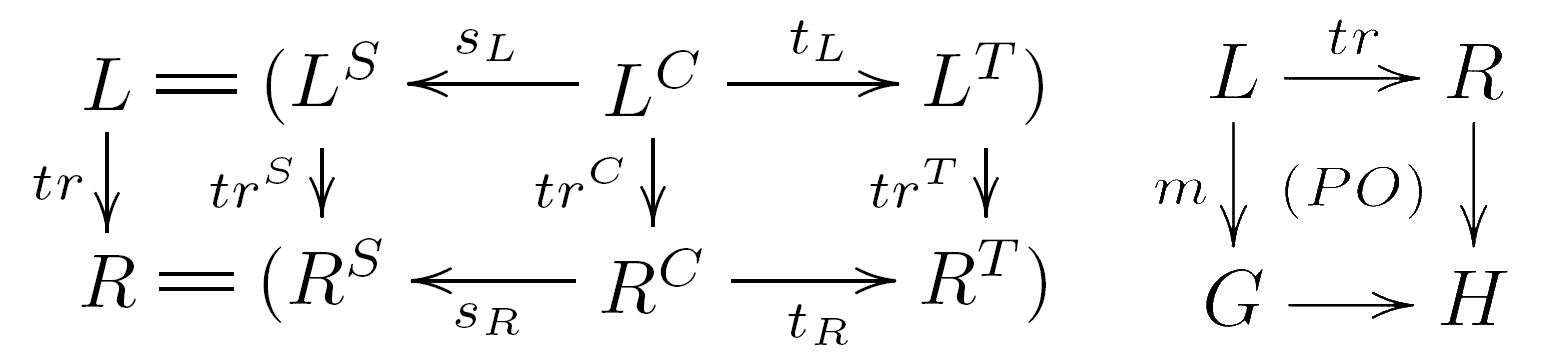
\includegraphics[width=8cm]{Tripelregel.png}
	\caption{Tripelregel und Tripeltransformationsschritt}
	\label{fig:Tripelregel}
\end{figure}

Gegeben sei ein Tripelgraphmorphismus $m:L \to G$. Dann ist ein \emph{Schritt}\index{Transformationsschritt} einer  \emph{Tripelgraphtransformation}\index{Tripelgraphtransformation}\index{TGT} (TGT)  $\xymatrix{G \ar@{=>}[r]^{tr,m} & H}$ (rechts in \autoref{fig:Tripelregel}) von $G$ nach $H$ durch den Pushout von Tripelgraphen mit Co-Match $n: R \to H$ und Transformation inclusion $t: G \hookrightarrow H$.
In \autoref{fig:Class2Table} ist eine Tripelregel für eine Beispielmodelltransformation CD2RDBM (ClassDiagram to DataBase Model) in verkürzter\footnote{die Verkürzung ist Abbildung von LHS und RHS in einem Grpahen durch <++>-Markierung} Notation abgebildet. LHS und RHS der Regel sind in einem Tripelgraph dargestellt. Elemente, die durch die Regel erstellt werden, sind mit einem grünen "`<++>"' markiert. Die Regel "`Class2Table"' erstellt eine Klasse mit dem Attribut name, dessen Wert "`cn"' ist, zusammen mit der entsprechenden Tabelle im relationalen Datenbankmodell.

\begin{figure}[h!] %{r}{6cm}
	\centering
	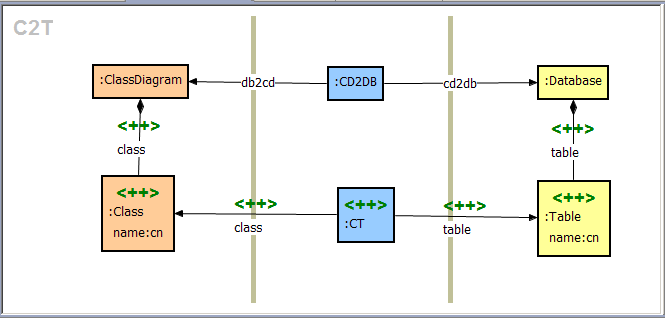
\includegraphics[width=12cm]{C2T}
	\caption{Beispiel Tripelregel: Class2Table}
	\label{fig:Class2Table}
\end{figure}

\subsubsection{Operationale Regeln}
Aus jeder Tripelregel $tr$ werden eine Sourceregel $tr_S$ für die Konstruktion von einem Modell der Sourcesprache und eine Forwardregel $tr_F$ für die Forward-Transformationsseqenz abgeleitet, wie in \autoref{fig:Sourceregel} und \autoref{fig:Forwardregel} gezeigt.

\begin{figure}[h!]%{r}{4cm}
	\centering
	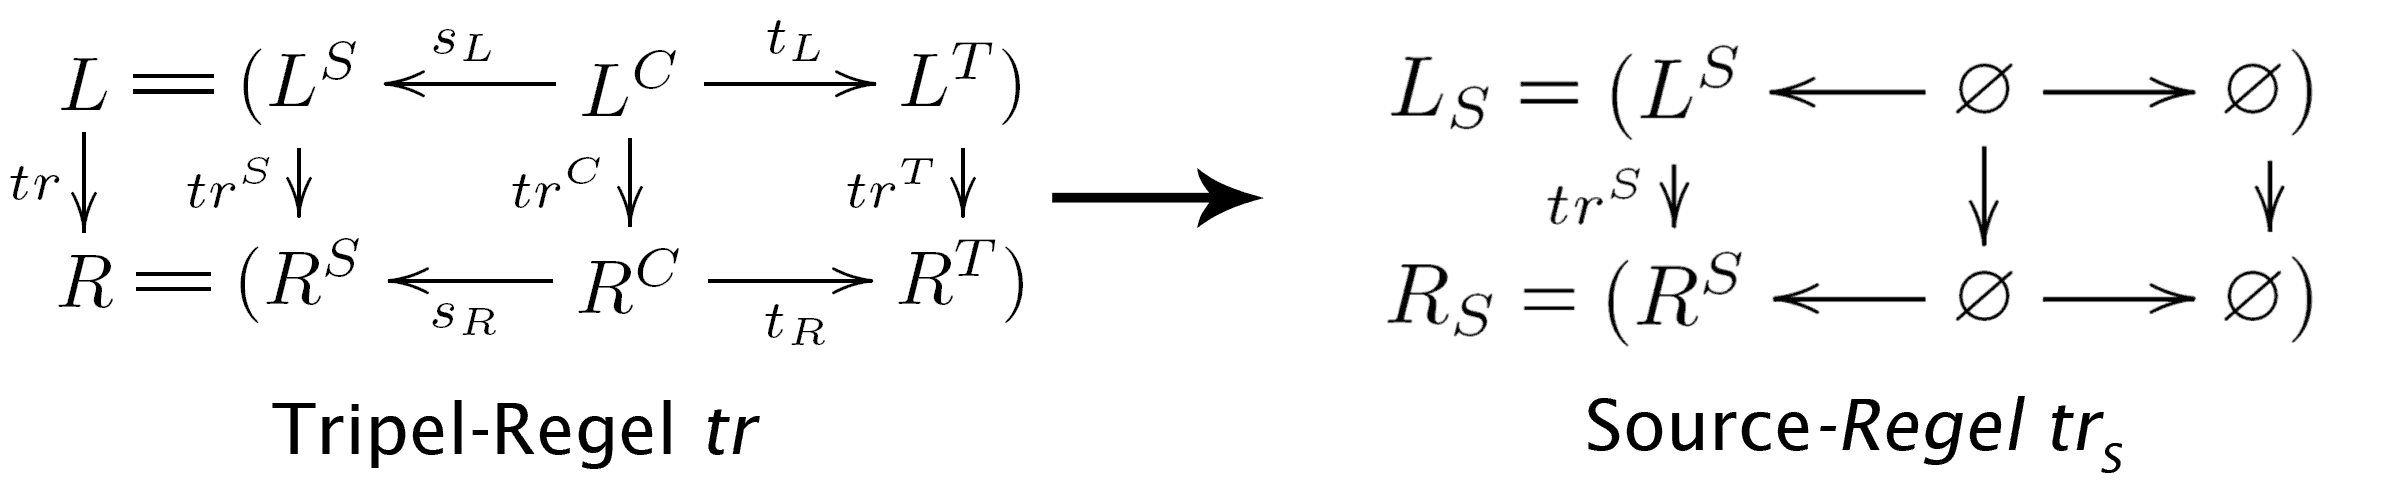
\includegraphics[width=10cm]{Sourceregel}
	\caption{Ableitung der Sourceregel}
	\label{fig:Sourceregel}
\end{figure}

\begin{figure}[h!]%{r}{4cm}
	\centering
	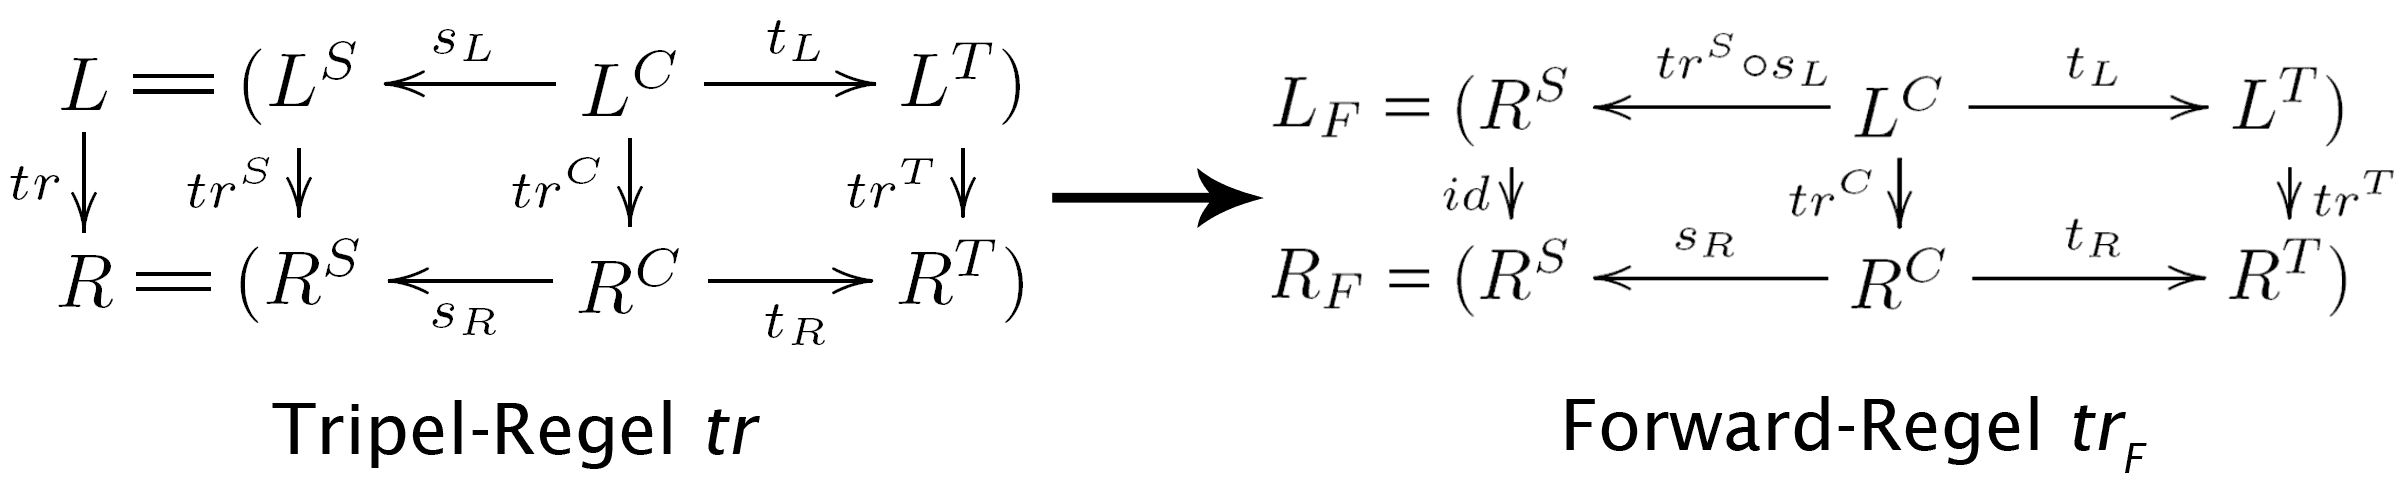
\includegraphics[width=10cm]{Forwardregel.png}
	\caption{Ableitung der Forwardregel $tr_F$}
	\label{fig:Forwardregel}
\end{figure}

In \autoref{fig:FT-Attribute2ForeignKey} wird die Forwardregel, die aus der Regel Attribute2ForeignKey abgeleitet wurde, als Beispiel gezeigt. Im Sourcegraphen sind die Elemente, die noch zu übersetzen sind, mit dem grünen Zeichen "`<tr>"' markiert.

\begin{figure}[h!]%{r}{4cm}
	\centering
	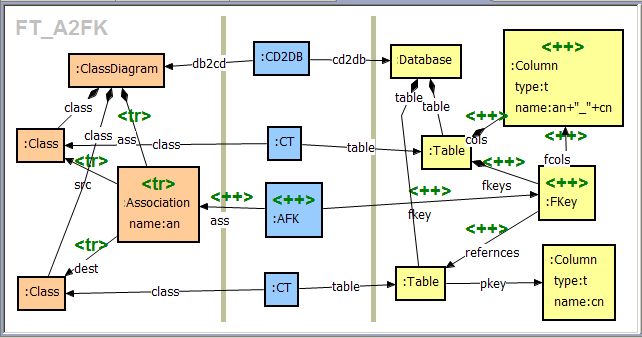
\includegraphics[width=12cm]{FT_A2FK.png}
	\caption{Beispiel Forwardregel: FT\_Attribute2ForeignKey}
	\label{fig:FT-Attribute2ForeignKey}
\end{figure}

\section{Ein paar Worte zur Implementation}\label{sec:implementation}
\subsection{Entwicklungsumgebung und Plugins}
Der Henshin TGG Editor ist als Plugin für Eclipse entwickelt worden und benötigt
die Plugins EMF und GEF. Die verwendeten Technologien werden im Folgenden
näher beschrieben.

\subsubsection{Eclipse}
\begin{wrapfigure}{r}{2cm}
	\centering
	
\includegraphics[width=2cm]{eclipse_logo}
%	\caption{Eclipse Logo}
	\label{fig:eclipse_logo}
\end{wrapfigure}
Eclipse\index{Eclipse}\footcite[][\url{http://www.eclipse.org/}]{eclipsewebsite}
%\footnote{Eclipse Webseite -http://www.eclipse.org/} ist eine Entwicklungsumgebung entwickelt von der Eclipse Foundation. Eclipse ist in Java
geschrieben und ist deswegen auch für die drei großen Betriebssysteme Windows,
Mac und Linux erhältlich. Eclipse ist kostenlos und Quell-offen. In erster Linie
wird Eclipse als Entwicklungsumgebung für Java verwendet. 

Wegen der Vielzahl an Plugins kann Eclipse aber auch für etliche andere Anwendungsfälle verwendet werden. So ist auch der TGG Editor ein Plugin von Eclipse.

\subsubsection{EMF}
\begin{wrapfigure}{r}{2cm}
	\centering
	
\includegraphics[width=2cm]{emf_logo}
%	\caption{EMF Logo}
	\label{fig:emf_logo}
\end{wrapfigure}
Das Eclipse Modeling Framework\index{Eclipse Modeling
Framework|see{EMF}}\index{EMF}\footcite[][\url{http://www.eclipse.org/modeling/emf/}]{emfwebsite}
%\footnote{EMF Webseite - http://www.eclipse.org/modeling/emf/} ist ein Plugin für Eclipse, das es ermöglicht Java Klassen 
grafisch ähnlich zu UML Klassendiagrammen zu modellieren. Aus einem so
entstandenen EMF Modell mit der Abkürzung .ecore kann automatisiert Java Code
generiert werden. Der Code kann dann weiter verwendet werden, um Instanzen des
Modells zu erstellen und zu manipulieren. EMF kann auch einen grundlegenden
grafischen Tree-Editor als Eclipse Plugin generieren. Der TGG Editor verwendet
das Henshin Modell, das mit EMF entwickelt wurde, und erweitert dieses mit
eigenen Klassen (siehe hierzu auch Abschnitt \ref{sec:henshin_modell}).

\subsubsection{GEF}
\begin{wrapfigure}{r}{2cm}
	\centering
	
\includegraphics[width=2cm]{gef_logo}
%	\caption{GEF Logo}
	\label{fig:gef_logo}
\end{wrapfigure}
Das Graphical Editing Framework\index{Graphical Editing
Framework|see{GEF}}\index{GEF}\footcite[][\url{http://www.eclipse.org/modeling/gef/}]{gefwebsite}
%\footnote{GEF Webseite - http://www.eclipse.org/modeling/gef/} ist ebenfalls ein Plugin für Eclipse, das
in der Model-View-Controller Architektur entwickelt wurde.
Mit GEF lassen sich sehr gut grafische Editoren als Plugins für Eclipse Entwickeln. GEF bietet 
ein Framework, damit der Entwickler grundlegende Funktionalitäten
eines grafischen Editors nicht von Grund auf implementieren muss.


So ist es in GEF relativ einfach grafische Objekte mit Verbindungen auf dem
Canvas zu zeichnen. Hier setzt GEF auf die Klassen des Packages
Draw2d\index{Draw2d}\footcite[][\url{http://www.eclipse.org/gef/draw2d/}]{draw2dwebsite}
%\footnote{Draw2d Webseite - http://www.eclipse.org/gef/draw2d/}.
GEF bietet weiter eine Palette mit Tools mit denen die grafischen Objekte
manipuliert werden können. Es ist außerdem durch GEF sehr einfach die Undo/Redo
für die einzelnen Operationen zu implementieren.
In unserem TGG Editor sind genau die Views\index{View} für Graphen und
Regeln mit den Tools in der Palette die GEF Editoren.

\subsubsection{MuvitorKit}
MuvitorKit\index{MuvitorKit} leitet sich ab von Multi-View-Editor-Plugin
ist ein Paket, das von Toni Modica an der TU Berlin entwickelt wurde. MuvitorKit
baut auf GEF auf und lässt es zu mehrere GEF Views in einer einzigen Page
anzuzeigen und zu editieren. Wir verwenden diese Funktionalität im TGG Editor
im Rule View\index{Rule View}. Denn hier werden zusätzlich NACs\index{NAC}
angezeigt und können editiert werden, falls die Regel NACs besitzt. Außerdem
verwenden wir im TGG Editor MuvitorKit für den Tree Editor\index{Tree Editor}.

\subsection{Das Henshin Metamodell und die Erweiterungen des TGG
Editors}\label{sec:henshin_modell}
\begin{figure}[htbp]
	\centering %bitte nicht center benutzen
	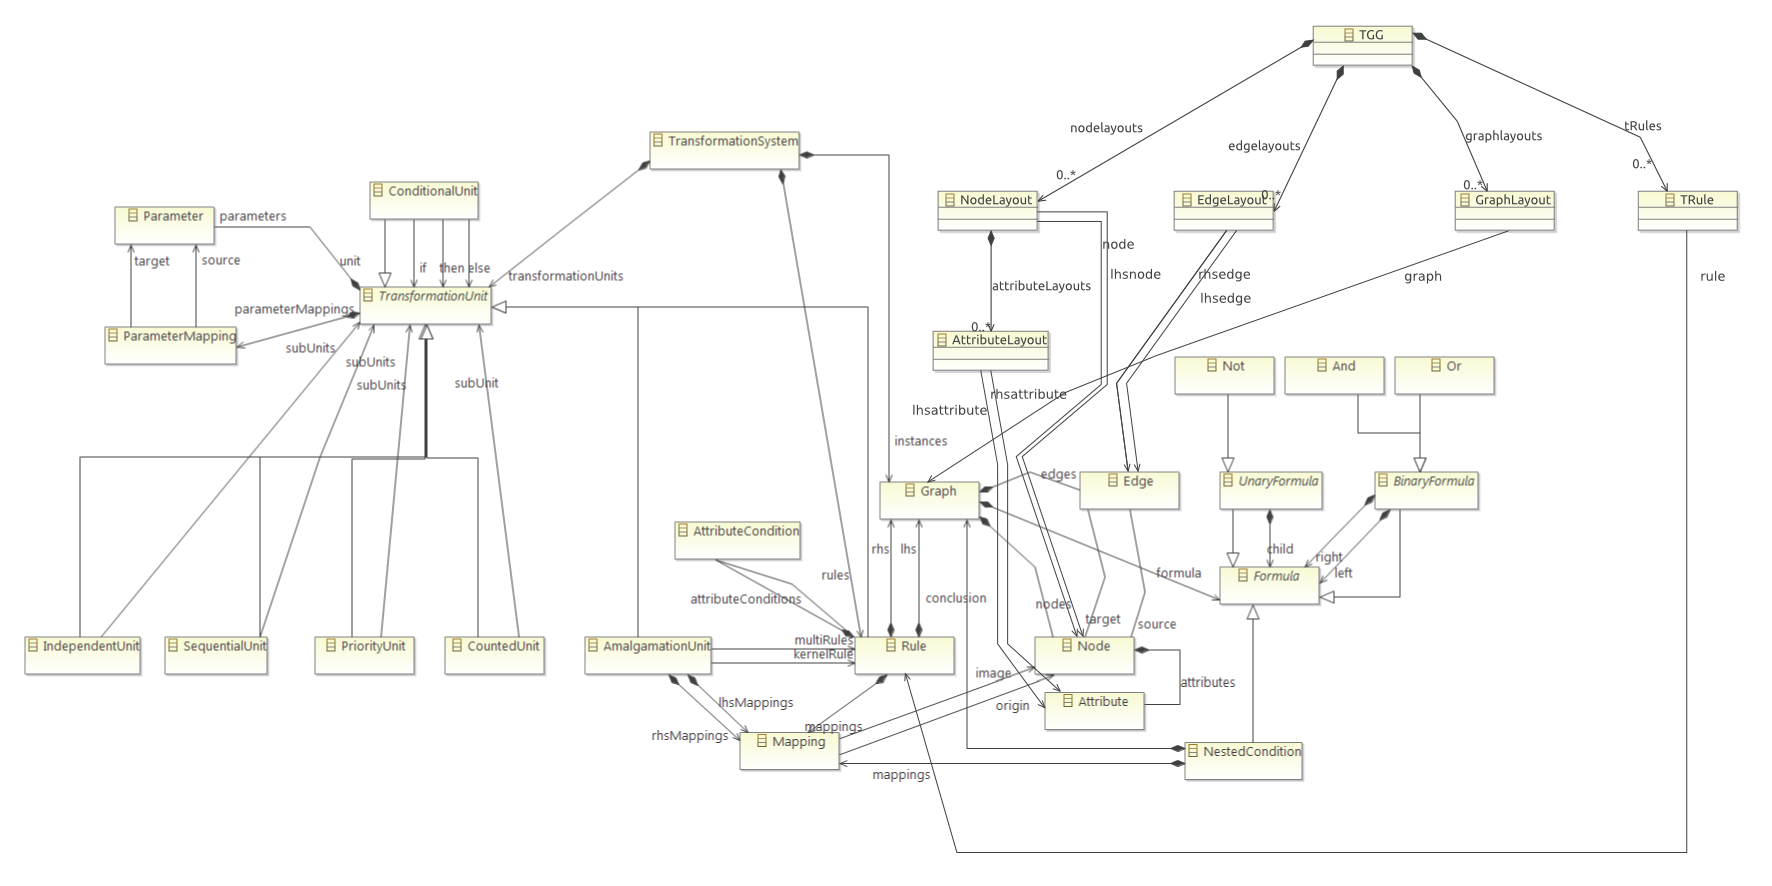
\includegraphics[width=\textwidth]{tgg_henshin_diagram}
	\caption[TGG Henshin Metamodell]{Das TGG Henshin Metamodell.}
	\label{fig:tgg_henshin_diagram}
\end{figure}

Der TGG Editor baut auf dem Henshin\index{Henshin Modell} Modell auf. Das in EMF\index{EMF} modellierte Henshin Modell wurde entwickelt für die allgemeineren Graphtransformationen. Für den TGG Editor wurden in einem eigenen EMF Modell alle nötigen Erweiterungen für Tripel Graph Grammatiken und Layoutinformationen gemacht. Die Klassen aus dem TGG Modell referenzieren die Klassen aus dem Henshin Modell nur. So bleibt das Henshin Modell unmodifiziert und macht Instanzen des Henshin Modells kompatibel zu anderen Editoren, die Instanzen des Henshin Modells verarbeiten können. In Abbildung \ref{fig:tgg_henshin_diagram} sind beide Modelle in einem Diagramm vereint. Das Diagramm gibt eine globale Sicht auf das gesamte Metamodell, das vom TGG Editor verwendet wird\footnote{Für diejenigen, die sich mit dem Henshin Modell näher auskennen ist noch hinzuzufügen, dass der TGG Editor TransformationUnits nicht benutzt. Es werden ausschließlich Graphen\index{Graph} und Rules\index{Rule} manipuliert. Außerdem können für Rules lediglich NACs\index{NAC} (NotApplicationCondition) und keine allgemeinen ACs erstellt werden, da dies bei Tripel Graph Grammatiken nicht unbedingt nötig ist.}.

\subsubsection{Die Erweiterungen für den TGG Editor}
\begin{figure}[htbp]
	\centering %bitte nicht center benutzen
	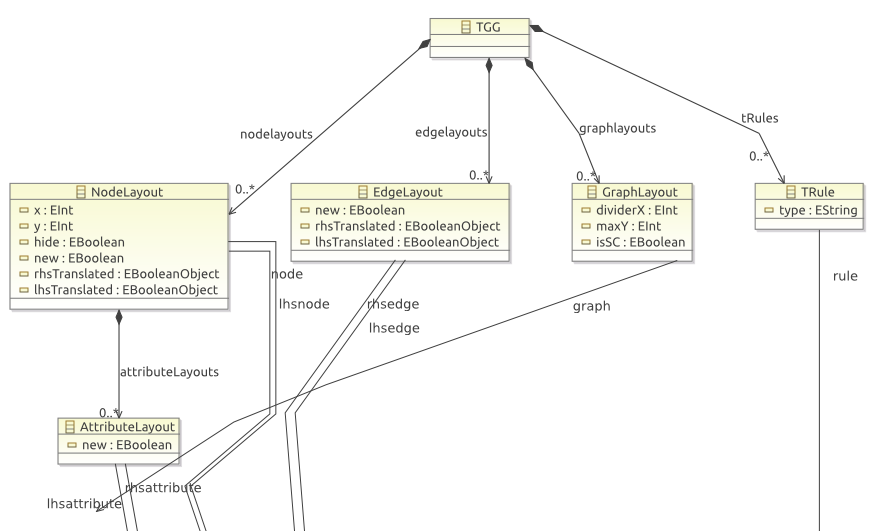
\includegraphics[width=\textwidth]{tgg_diagram}
	\caption[TGG Metamodell]{Das TGG Metamodell mit Attributen als Ausschnitt aus
	dem globalen Diagramm.}
	\label{fig:tgg_diagram}
\end{figure}

In diesem Abschnitt möchten wir auf das eigenständige EMF\index{EMF} Modell des TGG Editors etwas genauer eingehen. Die Klassen \emph{NodeLayout}, \emph{EdgeLayout}, \emph{GraphLayout}, \emph{TRule} und \emph{AttributeLayout} haben je eine Referenz zu den entsprechenden Klassen im Henshin Modell. Falls Instanzen einer Rule eine solche Layoutklasse haben gibt es je eine Referenz zur entsprechenden Instanz im LHS und RHS Graphen. So hat beispielsweise ein EdgeLayout für "`eine"'\footnote{Eigentlich sind es zwei Instanzen einer Edge, nämlich eine Edge im LHS Graphen und eine Edge im RHS Graphen. Im Rule View\index{Rule View} des TGG Editors wird die Edge allerdings nur als eine einzige Edge angezeigt. Siehe hierzu auch Abschnitt \ref{sec:ruleview}} Edge in einer Rule die Referenzen \emph{lhsedge} und \emph{rhsedge}.

\paragraph{NodeLayout}
Das \emph{NodeLayout} enthält nicht nur Layoutinformationen für einen Node sondern es hat auch noch weitere zusätzliche Attribute, die für Tripelgraphen benötigt sind. Die Attribute \emph{x} und \emph{y} geben die Position eines Nodes auf dem Canvas an. Für Knoten in einer Rule gibt es  das Attribut \emph{new}. Es zeigt an, ob ein Knoten mit einer Rule neu erstellt wird. Die Attribute \emph{rhsTranslated}\index{to be translated}\index{<tr>|see to be Translated} und \emph{lhsTranslated} sind lediglich für Nodes aus dem Sourceteil\index{Source} in einer FTRule\index{FTRule} bzw. TRule. Sie zeigen an, ob ein LHS bzw. RHS Node in einer FTRule als \emph{to be translated} markiert werden soll.
\paragraph{AttributeLayout}
Das \emph{AttributeLayout} hat ebenfalls das Attribute \emph{new}. Dieses Attribut ist äquivalent zu dem gleichnamigen Attribut aus dem NodeLayout.
\paragraph{EdgeLayout}
Die Attribute \emph{new}, \emph{rhsTranslated} und \emph{lhsTranslated} im \emph{EdgeLayout} entsprechen im wesentlich den gleichnamigen Attributen aus dem NodeLayout. Sie gelten nur eben für Edges.
\paragraph{GraphLayout}
Die Attribute \emph{dividerX} und \emph{maxY} sind Layoutinformationen für die Divider in den Views, die die einzelnen Teilgraphen Source, Correspondence und Target unterteilen.
\paragraph{TRule}
Wenn eine Instanz Rule von \emph{TRule} referenziert wird, dann ist die Rule keine normale Regel sonder eine FTRule\index{FTRule}. Das Attribute \emph{type} gibt den Typen einer Rule an, in diesem Fall nur FTRule, da andere Spezialregeln noch nicht implementiert sind.
